\section{Abstract Syntax Tree}
\label{abstract-syntax-tree}

Un \textit{abstract syntax tree}, nome spesso abbreviato utilizzando la sigla
AST, è uno strumento per la rappresentazione, sotto forma di albero, della
struttura di un programma.

Dal punto di vista formale, un abstract syntax tree è definito come un albero
ordinato ed etichettato, i cui nodi interni rappresentano gli operatori
utilizzati dal codice del programma che si desidera rappresentare e le cui
foglie rappresentano gli operandi soggetto delle operazioni precedentemente
citate. Un arco congiunge un nodo che rappresenta un operatore a ciascuno dei
suoi operandi o, eventualmente, agli operatori innestati a questo. Se si
considera un linguaggio di programmazione tradizionale, esempi di operatori sono
rappresentati da funzioni e operatori booleani, esempi di operandi sono
rappresentati da variabili e constanti.

Come affermato dalla precedente definizione, un AST rappresenta la struttura di
un programma. In particolare, a differenza di altri esempi di meccanismi di
rappresentazione, un AST fa riferimento alla \textit{struttura sintattica
astratta} di un programma.

La struttura sintattica astratta di un programma rappresenta un’astrazione
rispetto alla normale struttura, definita solitamente \textit{concreta} per
contrapposizione, di un linguaggio di programmazione. La sintassi astratta di un
linguaggio di programmazione si differenzia da quella concreta, utilizzata per
la scrittura di codice sorgente, in quanto solitamente ne rappresenta una
semplificazione. In particolare, la sintassi astratta non riporta tutte le
regole sintattiche che non influenzano la semantica del programma.

Un esempio di regola sintattica che viene trascurata dalla sintassi astratta di
un programma è rappresentata dalle \textit{grouping parentheses}, un costrutto
comune a diversi linguaggi di programmazione che consente di raggruppare un
certo insieme di elementi all'interno di un'unica espressione. La ragione per
cui questa particolare regola viene eliminata, all’interno della sintassi
astratta, è rappresentata dal fatto che questa non aggiunge alcuna informazione
rispetto alla semantica del programma. Infatti, l’informazione che l’utilizzo
delle parentesi trasmette, può essere trasmessa in maniera del tutto equivalente
semplicemente facendo riferimento ad una rappresentazione ad albero del
programma. Rappresentazione in cui elementi correlati possono essere raggruppati
dalla presenza un nodo antenato comune.

Un altro esempio di regola sintattica che viene trascurata per una ragione del
tutto equivalente è la regola di utilizzo del simbolo \texttt{;} come elemento
di separazione di un’istruzione dalla successiva. Anche in questo caso infatti
la struttura stessa dell’albero di rappresentazione suggerisce, attraverso i
nodi, la separazione di una data istruzione dalla successiva e può quindi essere
utilizzata per rappresentare la relazione di sequenzialità tra le istruzioni,
senza la necessità ulteriori modalità di rappresentazione.

Da un punto di vista pratico, un abstract syntax tree viene in molti casi
costruito a partire da un parse tree, definito anche \textit{concrete syntax
tree} nella letteratura. Un concrete syntax tree è una rappresentazione della
struttura sintattica concreta di un programma, prodotta tipicamente attraverso
il semplice e diretto parsing del codice sorgente. Il processo di generazione di
un AST a partire da un parse tree procede quindi per eliminazione di nodi e
archi ritenuti ridondanti o non necessari. Lo scopo di queste eliminazioni è
quello di ottenere una rappresentazione che possa servire come strumento più
comodo per le elaborazioni successive, uno strumento che non riporti
informazioni ridondanti o ritenute non interessanti per queste elaborazioni. Gli
AST sono infatti molto spesso degli strumenti per il supporto alla realizzazione
di funzionalità complesse e non un prodotto ultimo dell’elaborazione.

\begin{figure}
\makebox[\textwidth][c]{
  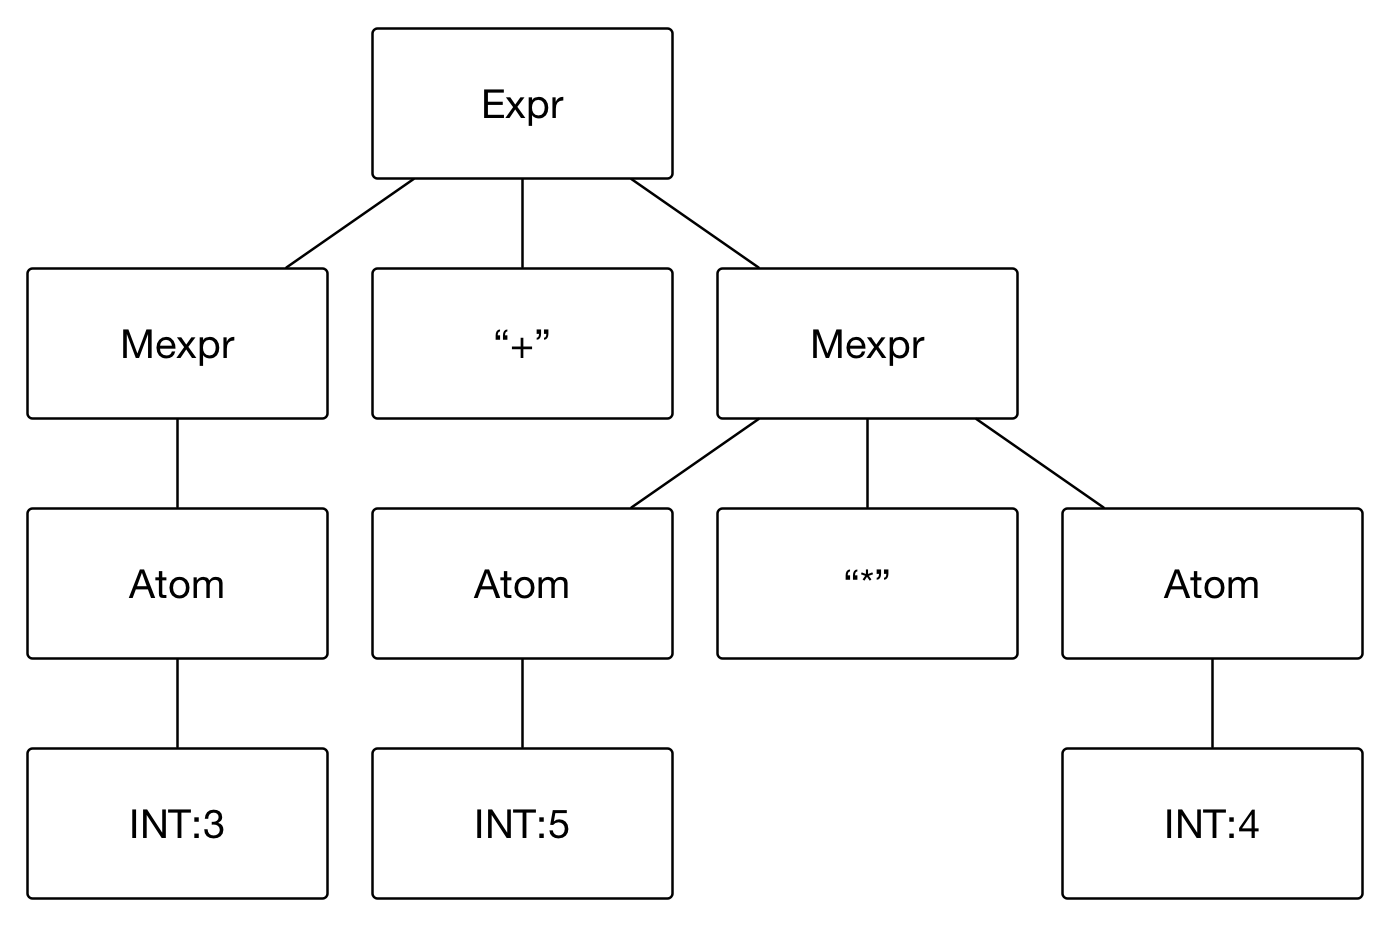
\includegraphics[scale=0.5]{img/concrete-syntax-tree.png}
}
\caption{Esempio di Concrete Syntax Tree per l'espressione \texttt{3 + 4 * 5}}
\label{fig:concrete-syntax-tree}
\end{figure}

\begin{figure}
\makebox[\textwidth][c]{
  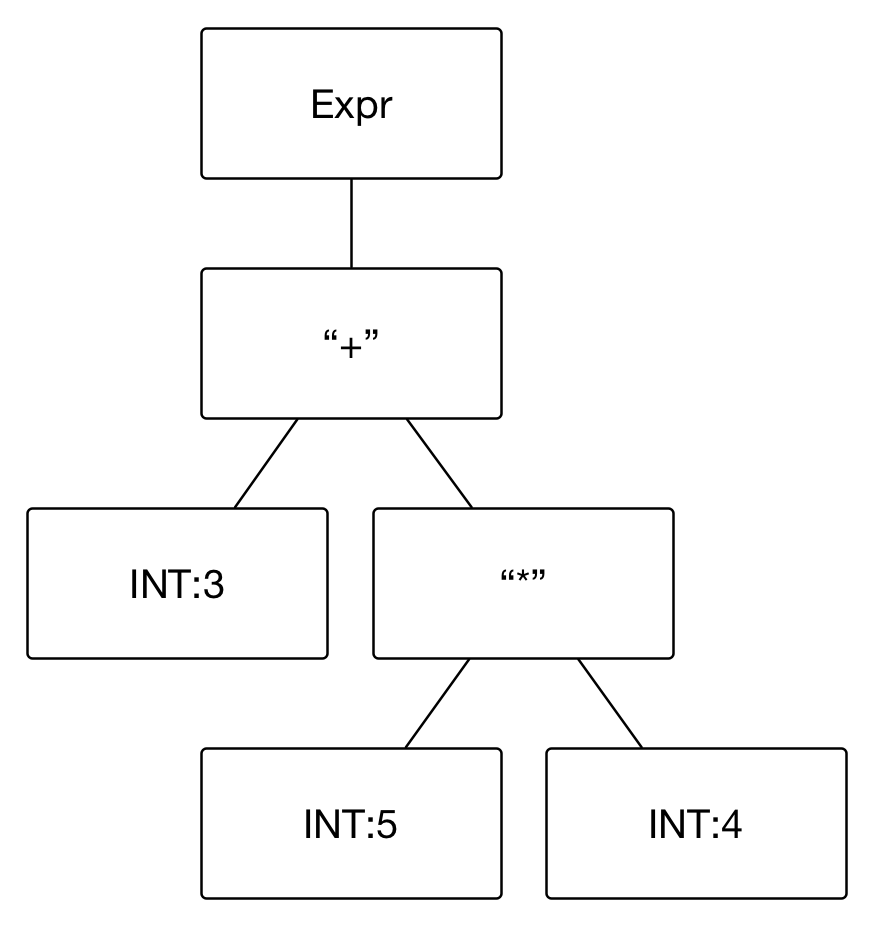
\includegraphics[scale=0.5]{img/abstract-syntax-tree.png}
}
\caption{Esempio di Abstract Syntax Tree per l'espressione \texttt{3 + 4 * 5}}
\label{fig:abstract-syntax-tree}
\end{figure}

Purtroppo, non esiste una tecnica per la generazione di AST indipendente dal
linguaggio e dal contesto di utilizzo. La causa fondamentale che porta a questa
mancanza di una strategia univoca è data proprio dalla natura di strumento di
supporto degli AST, natura a cui si è fatto riferimento nel paragrafo
precedente. Essendo un AST uno strumento di supporto, risulta infatti
particolarmente importante che questo venga definito a partire dalle necessità
caratteristiche delle funzionalità che si desidera realizzare a partire da
questo.

Molto spesso un AST viene quindi arricchito con informazioni aggiuntive e
caratteristiche del contesto di applicazione. Queste informazioni forniscono
maggiore conoscenza rispetto alla semantica del programma in modo specifico per
la funzionalità di ispezione o analisi per realizzare la quale si fa uso
dell’AST.

Riassumendo, il fatto che funzionalità diverse richiedono la disponibilità di
informazioni diverse e il fatto che gli AST nascono proprio come struttura per
favorire lo sviluppo di una certa funzionalità rendono poco ragionevole la
definizione di una strategia di generazione univoca.

La grande varietà di formalismi e costrutti che caratterizzano i diversi
linguaggi di programmazione e la velocità con la quale ne vengono introdotti di
nuovi rappresentano altri due fattori contribuirebbero a rendere un'ipotetica
strategia di generazione degli AST indipendente dal linguaggio poco efficace e
rapidamente obsoleta.

Come affermato nel corso dei paragrafi precedenti non risulta possibile, e
nemmeno particolarmente utile, definire una strategia di generazione degli ASTs
univoca. Un AST viene costruito in maniera specifica per un linguaggio di
programmazione e per la realizzazione di una specifica funzionalità.

Tuttavia, nel caso in cui si abbia una famiglia di linguaggi di programmazione
molto simili tra loro, ossia che condividono gran parte della propria sintassi
astratta, e si desideri realizzare una stessa funzionalità o uno stesso
strumento di analisi per ciascuno di questi, è possibile utilizzare un
rappresentazione unificata, comune a ciascuno dei linguaggi appartenenti alla
famiglia. Un AST di questo tipo, comune a diversi linguaggi di programmazione,
viene detto \textit{AST unificato}.

Formalmente, un AST unificato è una rappresentazione ad albero della struttura
sintattica astratta del codice sorgente di un programma scritto utilizzando un
linguaggio facente parte di una data famiglia di linguaggi di programmazione.

Un esempio di AST unificato è rappresentato dal clang AST, ossia l’Abstract
Syntax Tree che viene prodotto dallo strumento clang \footnote
{http://clang.llvm.org}, uno strumento che si pone come obiettivo quello di
definire un modulo di frontend per compilatore LLVM \footnote{http://llvm.org/},
compilatore comune alla famiglia di linguaggi di programmazione C, C++,
Objective C and Objective C++. \cite{DBLP:conf/lcpc/LattnerA04}

L’obiettivo più comune per il quale vengono impiegati gli AST è la
semplificazione e disaccoppiamento dei diversi passi che compongono il processo
di compilazione. Nelle prossime sezioni verrà brevemente illustrato il processo
con il quale un AST viene prodotto e utilizzato da un compilatore. Le
applicazioni degli AST non si limitano però al solo contesto dei compilatori;
nella letteratura è infatti possibile trovare applicazioni degli AST anche nel
contesto degli strumenti per il refactoring \cite{jscodeshift2016} e nel campo
della clone-detection \cite{DBLP:conf/saci/LazarB14}. Anche solamente
all’interno di un compilatore tuttavia, l’applicazione degli AST non si limita
al solo supporto della generazione di codice macchina. Altre applicazioni
all’interno di un compilatore vanno dal supporto per l'aggiunta di una
tipizzazione statica per il linguaggio target della compilazione a quello per
l'utilizzo di costrutti di pattern matching.

La libreria CLAST, soggetto di questa tesi, utilizza agli abstract syntax tree
come meccanismo per la rappresentazione di un programma al fine di consentire la
creazione di strumenti di source code analysis. Data quindi l'importanza, sia
dal punto di vista teorico che dal punto di vista pratico, di queste strutture
dati all'interno di CLAST, si è scelto di presentare, attraverso questa sezione,
un approfondimento rispetto alla teoria alla base degli AST e alle applicazioni
di questi nel contesto di strumenti per l'analisi ed elaborazione di sistemi
software.

La Sottosezione \ref{ast-applications} di questo capitolo fornisce una
panoramica delle principali applicazioni degli AST nei diversi contesti che
fanno un utilizzo di questo meccanismo di rappresentazione. Questo allo scopo di
introdurre il lettore ai requisiti che una libreria per la generazione di AST
per un linguaggio di programmazione, come la libreria CLAST descritta da questa
tesi, deve essere in grado di soddisfare.

\subsection{Applicazioni degli AST}
\label{ast-applications}

Le applicazioni degli abstract syntax tree sono diverse, sia nel mondo della
ricerca, sia nel mondo dei compilatori che nel mondo dell’industria. All’interno
di questa sezione vengono presentati alcuni esempi provenienti da questi
differenti mondi per sottolineare l’importanza della disponibilità di uno
strumento per la generazione di AST per un dato linguaggio di programmazione.
Questo consente quindi di mostrare al lettore l’utilità, i requisiti e la
tradizionale collocazione di uno strumento per la generazione di ASTs come
quello che viene trattato da questa tesi.

Essendo il maggiore campo di applicazione degli ASTs quello dei compilatori, nei
prossimi paragrafi se ne presenta un approfondimento.

\subsubsection{Nei compilatori}

L'obiettivo di un compilatore è quello di trasformare il proprio input,
rappresentato un programma scritto utilizzando un dato linguaggio di alto
livello, producendo come output una programma equivalente scritto in linguaggio
macchina. Tipicamente, il lavoro di un compilatore può essere scomposto in un
certo insieme di fasi in consecutive. Ciascuna di queste fasi riceve in input
una certa rappresentazione del programma originale e ne produce in output una
differente, arricchita e modificata al fine di consentire o semplificare le fasi
successive. In seguito, vengono presentate le fasi del processo di compilazione
che tipicamente portano alla generazione di un AST.

Le prime operazioni svolte durante il processo di compilazione sono quelle
relative all’analisi lessicale del codice sorgente, detta anche
\textit{scanning}. Lo scopo di questa fase è quello di leggere i caratteri che
compongono il codice sorgente del programma target della compilazione e riunirli
all’interno di gruppi logici di caratteri correlati tra loro detti
\textit{token}. Esempi di token comuni alla maggior parte dei linguaggi di
programmazione sono rappresentati dalle keyword utilizzate dal linguaggio, ossia
le sequenze di caratteri riservate dal linguaggio per identificare l'utilizzo di
particolari costrutti, i numeri interi e l’operatore di assegnamento. Una volta
identificati, i token vengono forniti come input alla fase successiva del
processo di compilazione in forma di stream.

La fase successiva alla fase di analisi lessicale è rappresentata dalla fase di
analisi sintattica o parsing, la quale fornisce, a partire dallo stream di token
prodotto dalla fase precedente, un insieme di entità sintattiche, come ad
esempio espressioni e istruzioni.

Le entità sintattiche sopraccitate vengono quindi poste, sempre durante questa
fase, all’interno di un parse tree, struttura a partire dalla quale viene
prodotto l’AST del programma, procedendo per eliminazione degli elementi
ridondanti o poco interessanti alle fasi successive, come affermato in apertura
di questa sezione nel corso della definizione di abstract syntax tree.

Nel caso di alcuni linguaggi di programmazione, la struttura sintattica target
del parsing risulta particolarmente semplice da trattare. In questi casi, alcuni
strumenti scelgono di non realizzare una fase di definizione del parse tree,
procedendo direttamente alla costruzione di un AST a partire dall’output della
fase di analisi sintattica.

All’interno di un compilatore, un abstract syntax tree rappresenta quindi molto
spesso l’output della fase di elaborazione compiuta dalla componente parser, o
più generalmente l’output della fase di parsing, e l’input per le successive
fasi di analisi semantica e generazione di codice macchina.

\begin{figure}
\makebox[\textwidth][c]{
  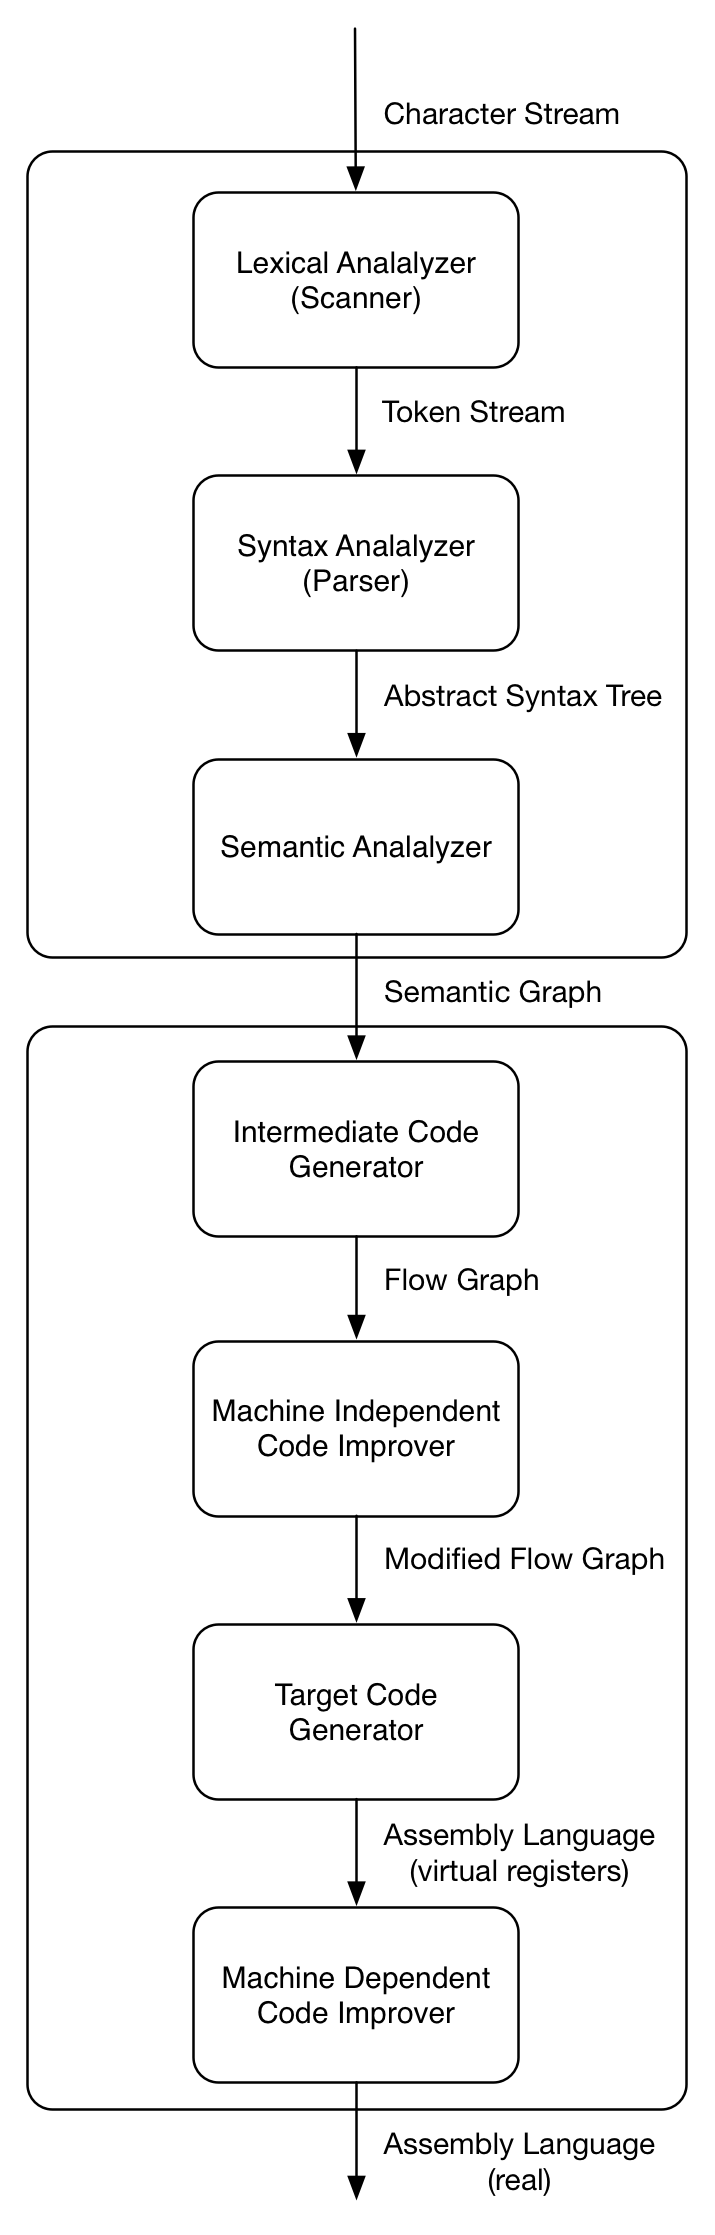
\includegraphics[scale=0.5]{img/compiler-architecture}
}
\caption{Architettura di un compilatore per un linguaggio di programmazione
tradizionale}
\label{fig:compiler-architecture}
\end{figure}

Tipicamente, un compilatore fa riferimento a diverse altre strutture dati
durante la sua azione. Tuttavia l’AST esegue ricopre un ruolo unico in quanto
utilizzato in moltissime fasi differenti, tra le quali:

\begin{itemize}

\item l'AST viene utilizzato molto intensamente durante la fase di analisi
semantica, durante la quale un compilatore verifica il corretto utilizzo degli
elementi del linguaggio e del programma.

\item Durante la fase di analisi semantica, un compilatore genera tabelle dei
simboli utilizzati da un programma a partire dall’AST.

\item Dopo essere stato utilizzato per la verifica della correttezza sintattica,
l’AST viene utilizzato come base per la generazione di codice macchina o, come
più spesso accade, viene utilizzato per la generazione di una ”intermediate
representation” o ”IR”, a cui spesso nella letteratura si fa riferimento come a
un linguaggio intermedio, apposito per la generazione di codice.

\end{itemize}

Dato l’elenco di operazioni svolte da un compilatore a partire da un AST,
riportato all’interno del paragrafo precedente, è possibile presentare alcuni
dei requisiti che vengono tipicamente a cui la progettazione e l’implementazione
di uno strumento per la generazione di AST sono soggette. É importante
sottolineare che, data la già citata natura di strumento di supporto degli AST,
specifici requisiti di un AST sono fortemente dipendenti dalla specifica
applicazione. Per questa ragione i requisiti presentati in seguito sono
solamente rappresentativi dell’applicazione del caso d'uso rappresentato dal
processo di compilazione di un linguaggio di programmazione tradizionale.

\begin{itemize}

\item La presenza di operatori n-ari in un linguaggio di programmazione rende
necessario che l’AST per tale linguaggio supporti la presenza di nodi con un
numero arbitrario di figli.

\item L’ordine di esecuzione delle istruzioni di un programma deve poter essere
correttamente identificato, conservato ed rappresentato in modo esplicito
dall’AST, come anche quello degli operandi di eventuali operazioni n-arie.

\item Gli identificativi e valori utilizzati dalle istruzioni di assegnamento
presenti all’interno del codice devono essere memorizzati e ricercabili tramite
ispezione dei nodi.

\item Durante la creazione dei nodi, i tipi delle variabili esplicitati dal
programmatore devono essere preservati, così come l'occorrenza di ciascuna
dichiarazione all’interno del codice sorgente.

\item A partire da un AST deve sempre essere possibile ricostruire il codice
sorgente originale nella sua interezza. Il codice prodotto in questo modo
dovrebbe essere sufficientemente simile al codice originale da conservarne il
funzionamento in fase di esecuzione, una volta ricompilato.

\end{itemize}

Data la complessità dei requisiti appena proposti in riferimento alla
progettazione di un AST per il compilatore di un dato linguaggio di
programmazione, l’applicazione di noti design pattern può risultare di grande
aiuto alla progettazione e  realizzazione di un sistema per la generazione di
ASTs.

Ad esempio, è fortemente probabile che un compilatore debba procedere diverse
volte alla visita dei nodi che compongono l’AST. Inoltre, molto spesso è
necessario che il compilatore svolga operazioni differenti a seconda dello
specifico tipo di nodo incontrato durante il processo di visita o in base al
valore di particolari attributi di questo. Infine, essendo un AST utilizzato da
diverse componenti di un compilatore, è importante che questo fornisca
un’interfaccia per la visita standard particolarmente facile da comprendere ed
utilizzare per tutti i differenti gruppi di progettisti e sviluppatori di queste
diverse componenti.

Un esempio di pattern che tradizionalmente risulta particolarmente appropriato
in questo contesto è rappresentato dal design pattern Visitor, presentato in
\cite{gamma1995design}. Il pattern Visitor risulta particolarmente appropriato a
questo contesto in quanto di soddisfare le necessità appena elencate, fornendo
delle linee guida che consentano facilmente l’implementazione delle operazioni
di visita dei singoli nodi e attraversamento dell’albero in modo efficiente,
fornendo accesso a tutte le informazioni relative a tipo e attributi a ciascuno
nodo, ed esponendo allo stesso tempo uninterfaccia tipicamente già familiare
agli utenti.

Dopo aver illustrato il principale campo di applicazione degli ASTs, e di
riflesso di uno strumento per la generazione di ASTs, la prossima sottosezione
di questo capitolo presenta alcuni dei principali lavori presenti nella
letteratura del settore rispetto a strumenti per la creazione, manipolazione ed
analisi degli AST, sottolineando alcune delle principali linee di ricerca in
questo ambito.

\subsubsection{Nella ricerca}
\label{ast-research}

In questa sottosezione vengono presentati alcuni lavori correlati allo strumento
presentato all’interno di questa tesi. Lo scopo di questa sottosezione è quindi
quello di fornire al lettore una panoramica rispetto ad alcuni dei campi di
applicazione di uno strumento per la generazione di AST nell'ambito della
ricerca. A questo scopo vengono elencati alcuni articoli relativi al mondo degli
abstract syntax tree, lavori che presentano il problema della progettazione di
AST e meccanismi di generazione per ASTs per la realizzazione di sistemi che
realizzano svariate funzionalità a partire dall’elaborazione delle informazioni
a cui questi danno accesso.

In \cite{martinez2014accurate}, Martinez et al. propongono una tecnica che
lavora a partire da un AST e, in particolare, basata sull’utilizzo di un
algoritmo di calcolo della distanza tra istanze di AST. Questa tecnica consente
la correzione di errori presenti a livello di codice sorgente mediante
l’identificazione di pattern di correzione precedentemente applicati durante lo
sviluppo.

La tecnica opera in prima battuta andando a ricercare all’interno di un sistema
per il controllo delle versioni tutte quelle revisioni che contengono la
correzione di un errore. Dopo questa prima fase di ricerca, il progetto viene
monitorato allo scopo di identificare nuove occorrenze di errori precedentemente
corretti. Ricerca e monitoraggio vengono entrambi operate a livello di AST,
utilizzando il sopraccitato algoritmo di calcolo della distanza tra AST. Una
volta identificata l’occorrenza di un errore precedentemente risolto, sempre
lavorando a livello di AST, viene applicata nuovamente la modifica identificata
come correzione per quel particolare errore.

ASTLOG è uno strumento sviluppato da Crew, durante il suo lavoro come
ricercatore presso Microsoft Inc. Si tratta di uno strumento che consente di
operare ricerche, anche molto complesse, all’interno del codice di un programma
scritto utilizzando i linguaggi C e C++, programmi anche di dimensioni molto
significative. \cite{DBLP:conf/dsl/Crew97}

Questo strumento si pone come alternativa ai generali metodi di ricerca in
sistemi UNIX come
grep\footnote{https://www.gnu.org/software/grep/manual/grep.html} e
awk\footnote{https://www.gnu.org/s/gawk/manual/gawk.html}, consentendo la
ricerca di pattern complessi come ad esempio: l’utilizzo di un particolare nome
di variabile, dichiarata specificando un dato tipo all’interno di un metodo che
prende in input un dato numero di parametri, presente all’interno di una classe
dichiarata all’interno di un file che importa una data libreria.

Lo strumento è stato realmente applicato anche al di fuori della ricerca e, in
particolare, \cite{DBLP:conf/dsl/Crew97} presenta come casi di studio ricerche
operate all’interno del codice sorgente di Microsoft SQL Server, descritto come
uno programma di 450mila righe di codice, e di Microsoft Word, ai tempi indicato
come un programma da più di due milioni di righe di codice.

In \cite{DBLP:conf/kbse/Welty97}, Welty presenta un’ontologia per la
rappresentazione di conoscenza a livello di codice sorgente basata sull’utilizzo
di ASTs. L’obiettivo di questa ontologia è quello di minimizzare lo sforzo
necessario ai singoli membri di un team di sviluppo per la documentazione e la
ricerca di informazioni relative all’implementazione di un sistema software,
strumenti grazie ai quali risulta più semplice l’aggiunta di nuovi membri ad un
team.

Bulychev e Minea descrivono, in \cite{peter2008duplicate}, un approccio,
indipendente dal linguaggio, per l’identificazione occorrenze di codice
duplicato, definite formalmente code clones dagli autori, all’interno di grandi
sistemi software. L’approccio viene quindi illustrato attraverso la
presentazione un algoritmo che consente di confrontare, a livello di AST, due o
più frammenti di codice al fine di ricercare sequenze di istruzioni che possono
essere riottenute, applicando le dovute sostituzioni di sottoalberi agli AST, a
partire dalle sequenze di istruzioni presenti all’interno di altri frammenti di
codice.

Utilizzando come fondamento il lavoro di Bulychev e Minea, Lazar e Banias
presentano una metodologia \cite{DBLP:conf/saci/LazarB14} per l’identificazione
di episodi di plagio nello specifico contesto di sistemi software sviluppati
utilizzando il linguaggio di programmazione C. Uno degli elementi di maggiore
interesse esposti da questo lavoro, rispetto ai contenuti di questa tesi, è
rappresentato dallo studio che i due autori descrivono rispetto alle riflessioni
operate per la definizione del meccanismo di generazione degli AST. Gli autori
presentano infatti la descrizione di un meccanismo, esterno al processo di
compilazione, costruito in maniera tale da riportare solamente gli elementi
strettamente necessari all’analisi che la metodologia si pone come obiettivo.

In \cite{DBLP:conf/acsac/YamaguchiLR12}, Yagamaguchi et al. descrivono una
tecnica per l’analisi di AST al fine di identificare pattern riconosciuti
durante lo studio di vulnerabilità software note. Questo al fine di poter
verificare la presenza di occorrenze di queste stesse vulnerabilità ed
eventualmente segnalare le modifiche necessarie che lo sviluppatore del sistema
dovrà applicare.

Infine, Neamtiu et al. descrivono in \cite{DBLP:journals/sigsoft/NeamtiuFH05}
uno strumento che lavora combinando un sistema di controllo delle versioni ad
un’analisi degli AST e che consente di tracciare e studiare l’evoluzione nel
tempo di un sistema software, scritto utilizzando il linguaggio C, soprattutto
per quanto concerne gli aspetti architetturali del sistema.

\subsubsection{Nell’industria}

Mentre la precedente sottosezione ha elencato alcuni degli utilizzi degli AST
nel mondo della ricerca, all’interno di questa sottosezione vengono presentate
alcune delle applicazioni degli AST che possono essere rintracciate nel mondo
dell’industria. Questo al fine di completare la panoramica che questo capitolo
ha offerto sui requisiti e sulle applicazioni degli abstract syntax tree e dei
sistemi per la loro generazione.

Dopo alla più tradizionale applicazione degli AST, illustrata nella sottosezione
di questo capitolo dedicata all’utilizzo degli AST nel contesto di un
compilatore, la seconda applicazione più significativa degli AST è all’interno
di strumenti per il supporto allo sviluppo, in particolare all’interno di
sistemi per l'analisi e modifica di codice sorgente.

Per molti programmatori, la possibilità di utilizzare all’interno del proprio
IDE una funzionalità che consenta di selezionare un insieme di istruzioni e
costruire un metodo a partire da queste, tipicamente chiamata \texttt{Extract
Method}, è una funzionalità la cui presenza viene data sostanzialmente per
scontata.

Perché sia possibile realizzare questa funzionalità, e più generalmente perché
sia possibile realizzare un sistema che consenta di svolgere una qualsiasi
operazione di refactoring, è però di fondamentale importanza avere a
disposizione un meccanismo di rappresentazione del codice del sistema in
analisi. Gli AST rappresentano la struttura dati più appropriata, e più
impiegata \cite{eclipse2006} \cite{netbeans2007}, a questo scopo.

Eclipse\footnote{https://www.eclipse.org}, l’IDE più utilizzato dagli utenti del
linguaggio di programmazione Java, realizza la funzionalità appena descritta e,
più generalmente la grande maggioranza delle operazioni di modifica di codice
sorgente automatica, a partire da ASTParser, una libreria Java che consente la
generazione e visita dell’abstract syntax tree di un programma. Libreria che è
possibile utilizzare anche per la generazione di plugin che estendono le
funzionalità dell’ambiente Eclipse stesso da parte di sviluppatori di terze
parti.

JSCodeshift \cite{jscodeshift2016} è un altro esempio di strumento che utilizza
come fondamento per il suo funzionamento gli abstract syntax tree. JSCodeshift
è uno strumento open-source, nato come progetto interno a Facebook\texttrademark,
per la manutenzione di grandi quantità di codice JavaScript.

In particolare, JSCodeShift viene utilizzato per operare \textit{codemod},
termine con il quale gli sviluppatori dello strumento fanno riferimento ad un
insieme di cambiamenti su larga scala che coinvolgono grandi porzioni di del
codice di un sistema. Cambiamenti che possono consistere di semplici modifiche,
come ad esempio la sostituzione del nome di una variabile o metodo, o anche di
modiche molto complesse, come l'aggiornamento delle chiamate ad una libreria o
interazione con un framework a seguito di cambiamenti critici, \textit{source
breaking changes}, nell'interfaccia o funzionamento di questo.

Da un punto di vista pratico, il funzionamento di JSCodeshift può essere
semplificato come segue: lo strumento prende in input un frammento di codice
JavaScript ed il mapping associato alla modifica che si desidera venga operata
dallo strumento, e produce in output un nuovo frammento di codice JavaScript in
cui il mapping è stato applicato a tutte le occorrenze del pattern di input
associato alla modifica. Mapping che descrive, a livello di AST, la modifica che
si desidera venga applicata al codice matchato da una particolare espressione di
origine specificata per esso.

Lo strumento lavora quindi completamente a livello di AST andando dapprima a
generare l’AST del codice in input, andando poi ad identificare i nodi
all’interno di questo che sono matchati dall’espressione di origine del mapping,
generando codice di rimpiazzo adeguato a partire dal nodo matchato e dal mapping
fornito in input, operando il rimpiazzo del nodo, e andando infine a rigenerare
codice JavaScript a partire dall’AST all’interno del quale è stata operata la
sostituzione.

Nonostante la relativa semplicità dello strumento dal punto di vista
concettuale, la sua utilità risulta molto significativa. Consente infatti di
operare modifiche anche molto complesse a sistemi software di grandi dimensioni
\cite{jsconf2016}. Modifiche che risulterebbero eccessivamente dispendiose in
termini di tempo, qualora operate in modo manuale, o addirittura impossibili
utilizzando approcci più tradizionali come ad esempio quelli basati su
espressioni regolari, questo soprattutto a causa della presenza di costrutti
ambigui nella, sempre in evoluzione, grammatica del linguaggio JavaScript.
